% !TeX spellcheck = en_GB
\documentclass[a4paper, 11pt]{article}
\usepackage[english]{babel}
\usepackage{newtxtext,newtxmath}

\usepackage{amsmath}
\usepackage{mathtools}
\usepackage{dramatist}
\usepackage{dirtytalk}
\usepackage{multicol}
\usepackage{soul}
\usepackage{xcolor}

\usepackage[round]{natbib}

\usepackage{geometry}
\geometry{
	a4paper,
	total={150mm,257mm},
	top=20mm,
}

\usepackage{hyperref}
\hypersetup{
	colorlinks=true,
	linkcolor=blue,
	filecolor=blue,      
	urlcolor=blue,
	citecolor=blue
}

\setlength\parindent{0pt}

%opening
\title{\textbf{Natural Language Processing}\\Portfolio I}
\author{\textbf{Leon F.A. Wetzel}\\ Information Science \\ Faculty of Arts - University of Groningen\\ \texttt{l.f.a.wetzel@student.rug.nl}}

\begin{document}

\maketitle

\begin{abstract}
	
	In this document, you can find the results and explanations for the assignments of the first part of the portfolio for the course Natural Language Processing, taught at the University of Groningen. The corresponding Python code can be found at \url{https://github.com/leonwetzel/natural-language-processing}\footnote{All code will be published after the course has been completed}. Note that version control of Jupyter notebooks is done via \texttt{jupytext}, so do not forget to convert the relevant Python scripts to notebooks yourself!

\end{abstract}

\section{Week 1 - Regular Expressions}

We used \url{https://regex101.com/} to test our regular expressions. In this document, we use \texttt{$\wedge$} to better display/represent a caret. Spaces cannot be displayed in \LaTeX  sadly, so these are not shown below.

\subsection{Regular Expressions I}

\begin{enumerate}
	\item Set of all alphabetic strings. \\ $ \wedge [a-zA-z ]+\$ $
	
	\item Set of all lower case alphabetic strings ending in $b$. \\ $\wedge [a-z ]*[b]\$ $
	
	\item Set of all strings from the alphabet ${a,b}$ such that each $a$ is immediately preceded by a $b$ and immediately followed by a $b$. \\$\wedge(bab)+\$ $
\end{enumerate}

\subsection{Regular Expressions II}

\begin{enumerate}
	\item Set of all strings with two consecutive repeated words (e.g., \textit{“Humbert Humbert”} and \textit{“the the”} but not \textit{“the bug”} or \textit{“the big and the bug”}). \\ $ \textbackslash b(\textbackslash w+)\textbackslash b \textbackslash s+ \textbackslash1 $
	
	\item All strings that start at the beginning of the line with an integer and that end with a word. \\ $ \wedge \textbackslash d+.+ \textbackslash b[a-zA-Z]+\textbackslash b \$ $
	
	\item All strings that have both the word \textit{grotto} and the word \textit{raven} in them (but not, e.g., words like \textit{grottos} that merely contain the word \textit{grotto}). \\ $ \textbackslash b \space { grotto} \textbackslash b.* | \textbackslash b \space { raven} \textbackslash b.*  $
\end{enumerate}

\subsection{ELIZA}

We added extra regular expressions and substitutions to handle more variants of user input. We also implemented a substitution to handle question marks, so that ELIZA's responses feel more like proper questions when relevant. The other implemented substitutions are related to how one feels, and takes into account words such as \textit{encounter}, \textit{experience} and \textit{suffer from}. Snippets from example dialogue can be found below.

\begin{drama}
	\Character{ELIZA}{eliza}
	\Character{Leon}{leon}
	
	\elizaspeaks: How are you?  
	
	\leonspeaks: I experience coldness.
	
	\elizaspeaks: Why do you experience coldness?
	
	\leonspeaks: I feel as if it is snowing today
	
	\elizaspeaks: Why do you feel as if it is snowing today?
	
	\leonspeaks: Because it is snowing today
	
	\elizaspeaks: Because it is snowing today?
	
	\leonspeaks: Yes, but I am inside
	
	\elizaspeaks: Yes, but Why are you inside?
	
	\leonspeaks: Because it is cold outside
	
	\elizaspeaks: Because it is cold outside?
	
	\leonspeaks: Yes
	
\end{drama}

\subsection{Byte-Pair Encoding}

Our example text for the experiment is a snippet from the Wikipedia page on the GameStop short squeeze\footnote{\url{https://en.wikipedia.org/wiki/GameStop_short_squeeze}}, which occurred in January 2021. According to \url{https://wordcounter.net}, our example consists of 137 words and 827 characters.\\

"\textit{In January 2021, a short squeeze of the stock of the American video game retailer GameStop (NYSE: GME) and other securities took place, causing major financial consequences for certain hedge funds and large losses for short sellers. Approximately 140 percent of GameStop's public float had been sold short, and the rush to buy shares to cover those positions as the price rose caused it to rise even further. The short squeeze was initially and primarily triggered by users of the subreddit r/wallstreetbets, an Internet forum on the social news website Reddit. At its height, on January 28, the short squeeze caused the retailer's stock price to reach a pre-market value of over US\$500 per share, nearly 30 times the \$17.25 valuation at the beginning of the month. The price of many other heavily shorted securities increased.}"\\

The default value for \texttt{vocab\_size} ($v$) is $30000$. With this value, we can count 164 words and 190 segments found in our example text by the tokenizer. For $v=25000$, we count 164 words and 195 segments, and the counts for $v=20000$ are 164 words and 197 segments. In line with the assignment description, we can observe here that more words are segmented into subwords when the number of segments increase (as a result of $v$ decreasing). An overview of the results can be found in table \ref{tab:tokenizer_results}.

\begin{table}[h]
	\centering
	\begin{tabular}{l|l|l|l|l|l|l|l|l}
	$v$		 & 30000 & 25000 & 20000  & 15000 & 10000 & 7500 & 5000 & 2500\\ \hline
	Words 	 & 164 	 & 164   & 164    & 164   & 164   & 164  & 164  & 164\\ 
	Segments & 190   & 195   & 197    & 204	  & 222   & 246  & 692  & 692
	\end{tabular}
	\caption{Overview of \texttt{vocab\_size} values and the word and segment counts}
	\label{tab:tokenizer_results}
\end{table}

When $v=7500$, the number of segments (246) is exactly 150\% of the number of words (164). The longest words in our example text during this setup that were not segmented, are \textit{increased}, \textit{beginning} and \textit{initially}. All these words consist of nine characters each.

\section{Week 2 - N-gram Language Models}

For this week's assignment, we take a look at several exercises from \citet{jurafskyspeech}.

\subsection{J\&M exercise 3.1}

\noindent\fbox{%
	\parbox{\textwidth}{%
Write out the equation for trigram probability estimation (modifying Eq. 3.11). Now write out all the non-zero trigram probabilities for the I am Sam corpus on page 41.
	}%
}\\


The original - simplified - formula for bigram probability estimation is as follows:

$$P(w_{n} | w_{n-1}) = \frac{C(w_{n-1}w_{n})}{C(w_{n-1})}$$

For trigram probability estimation, the formula would be:

$$P(w_{n} | w_{n-2} w_{n-1}) = \frac{C(w_{n-2} w_{n-1}w_{n})}{C(w_{n-2} w_{n-1})}$$

Our corpus contains the following sentences:

\texttt{<s> I am Sam </s> \enspace <s> Sam I am </s> \enspace <s> I do not  like green eggs and ham </s>}\\

The non-zero trigram probabilities would be:

\begin{multicols}{2}
	\noindent
	\begin{equation}
P(\text{Sam} | \text{I am}) = \frac{C(\text{I am Sam})}{C(\text{I am})} = \frac{1}{2} = 0.5
	\end{equation}
	\begin{equation}
P(\text{am} | \text{<s> I}) = \frac{C(\text{<s> I am})}{C(\text{<s> I})} = \frac{1}{2} = 0.5
	\end{equation}
	\begin{equation}
	P(\text{</s>} | \text{am Sam}) = \frac{C(\text{am Sam </s>})}{C(\text{am Sam})} = \frac{1}{1} = 1.0
	\end{equation}
	\begin{equation}
	P(\text{I} | \text{<s> Sam}) = \frac{C(\text{<s> Sam I})}{C(\text{<s> Sam})} = \frac{1}{1} = 1.0
\end{equation}
	\begin{equation}
	P(\text{am} | \text{Sam I}) = \frac{C(\text{Sam I am})}{C(\text{Sam I})} = \frac{1}{1} = 1.0
\end{equation}
	\begin{equation}
	P(\text{</s>} | \text{I am}) = \frac{C(\text{I am </s>})}{C(\text{I am})} = \frac{1}{2} = 0.5
\end{equation}
	\begin{equation}
	P(\text{do} | \text{<s> I}) = \frac{C(\text{<s> I do})}{C(\text{<s>I})} = \frac{1}{2} = 0.5
\end{equation}
	\begin{equation}
	P(\text{not} | \text{I do}) = \frac{C(\text{I do not})}{C(\text{I do})} = \frac{1}{1} = 1.0
\end{equation}
	\begin{equation}
	P(\text{like} | \text{do not}) = \frac{C(\text{do not like})}{C(\text{do not})} = \frac{1}{1} = 1.0
\end{equation}
	\begin{equation}
	P(\text{green} | \text{not like}) = \frac{C(\text{not like green})}{C(\text{not like})} = \frac{1}{1} = 1.0
\end{equation}
	\begin{equation}
	P(\text{eggs} | \text{like green}) = \frac{C(\text{like green eggs})}{C(\text{like green})} = \frac{1}{1} = 1.0
\end{equation}
	\begin{equation}
	P(\text{and} | \text{green eggs}) = \frac{C(\text{green eggs and})}{C(\text{green eggs})} = \frac{1}{1} = 1.0
\end{equation}
	\begin{equation}
	P(\text{ham} | \text{eggs and}) = \frac{C(\text{eggs and ham})}{C(\text{eggs and})} = \frac{1}{1} = 1.0
\end{equation}
	\begin{equation}
	P(\text{</s>} | \text{and ham}) = \frac{C(\text{and ham </s>})}{C(\text{and ham})} = \frac{1}{1} = 1.0
\end{equation}
\end{multicols}

\subsection{J\&M exercise 3.2}

\noindent\fbox{%
	\parbox{\textwidth}{%
Calculate the probability of the sentence \textit{i want chinese food}. Give two probabilities, one using Fig. 3.2, and another using the add-1 smoothed table in Fig. 3.6.
	}%
}\\

Our sentence is:
\texttt{<s> i want chinese food </s>}\\

The formula and result using figure 3.2 would be:
\begin{equation}
	\begin{split}
		P(\text{<s> i want chinese food </s>}) & = P(\text{i}|\text{<s>}) * P(\text{want}|\text{i}) * P(\text{chinese}|\text{want}) * P(\text{food}|\text{chinese}) * P(\text{</s>}|\text{food}) \\
		& = 0.25 * 0.33 * 0.0065 * 0.00092 * 0.68 \\
		& = \textbf{0.00000034}
	\end{split}
\end{equation}

The formula and result using the add-1 smoothness from figure 3.6 would be:
\begin{equation}
	\begin{split}
		P_{\text{Laplace}}(\text{<s> i want chinese food </s>}) & = P_{\text{Laplace}}(\text{i}|\text{<s>}) * P_{\text{Laplace}}(\text{want}|\text{i}) * P_{\text{Laplace}}(\text{chinese}|\text{want}) \\& * P_{\text{Laplace}}(\text{food}|\text{chinese}) * P_{\text{Laplace}}(\text{</s>}|\text{food}) \\
		& = 0.25 * 0.21 * 0.0029 * 0.052 * 0.68 \\
		& = \textbf{0.00000538356}
	\end{split}
\end{equation}


\subsection{J\&M exercise 3.6}

\noindent\fbox{%
	\parbox{\textwidth}{%
Suppose we train a trigram language model with add-one smoothing on a given corpus. The corpus contains $V$ word types. Express a formula for estimating $P(w3|w1,w2)$, where $w3$ is a word which follows the bigram $(w1,w2)$, in terms of various N-gram counts and $V$. Use the notation $c(w1,w2,w3)$ to denote the number of times that trigram $(w1,w2,w3)$ occurs in the corpus, and so on for bigrams and unigrams.
	}%
}\\

The original formula with Laplacian smoothing is:

\begin{equation}
	P_{\text{Laplace}}(w_i) = \frac{c_i + 1}{N + V}
\end{equation}

A similar formula supporting trigrams would look like:

\begin{equation}
	P^*_{\text{Laplace}}(w_n|w_{n-1} w_{n-2}) = \frac{C(w_{n-2}w_{n-1}w_{n})+1}{\sum_{w} (C(w_{n-2}w_{n-1}w) + 1)} = \frac{C(w_{n-2}w_{n-1}w_n) + 1}{C(w_{n-2}w_{n-1}) + V}
\end{equation}

\subsection{J\&M exercise 3.7}

\noindent\fbox{%
	\parbox{\textwidth}{%
We are given the following corpus, modified from the one in the chapter:\\
\texttt{<s> I am Sam </s>\\
<s> Sam I am </s>\\
<s> I am Sam </s>\\
<s> I do not  like green eggs and Sam </s>\\}
If we use linear interpolation smoothing between a maximum-likelihood bi-gram model and a maximum-likelihood unigram model with $\lambda1 = 1/2$ and $\lambda2 = 1/2$ , what is $P(\text{Sam}|\text{am})$? Include <s> and </s> in your counts just like any other token.
	}%
}\\

By the use of linear interpolation smoothing between the maximum-likelihood n-gram models (with $\lambda_{1} = 1/2$ and $\lambda_{2} = 1/2$), the formula would look like:

\begin{equation}
	\begin{split}
		\hat{P}(w_n|w_{n-1}) = \lambda_1 P(w_n|w_{n-1}) + \lambda_2 P(w_{n})
	\end{split}
\end{equation}

\begin{equation}
	\begin{split}
		\hat{P}(\text{Sam}|\text{am}) & = 1/2 * P(\text{Sam}|\text{am}) + 1/2 * P(\text{Sam}) \\
		 & = 1/2 * \frac{C(\text{am Sam}) + 1}{C(\text{am}) + 1} + 1/2 * \frac{C(\text{am}) + 1}{C(\text{am}) + 1} \\ & = 1/2 * \frac{2 + 1}{3 + 1} + 1/2 * 1
		 \\ & = 0.375 + 0.5 \\ & = 0.875
	\end{split}
\end{equation}

\subsection{N-grams in the notebook}

\noindent\fbox{%
	\parbox{\textwidth}{%
What are the different and common n-grams? You may ignore n-grams containing punctuation symbols.
	}%
}\\

We looked for common and different n-grams between the speeches of Theodore Roosevelt and Franklin D. Roosevelt. The common bigrams are:

\texttt{ ('can', 'not'), ('is', 'the'), ('the', 'country'), ('have', 'been'), ('there', 'is'), ('of', 'the'), ('to', 'make'), ('the', 'people'), ('that', 'the'), ('and', 'to'), ('is', 'a'), ('the', 'other'), ('of', 'a'), ('and', 'in'), ('in', 'this'), ('the', 'same'), ('they', 'are'), ('is', 'not'), ('has', 'been'), ('it', 'is'), ('with', 'the'), ('and', 'the'), ('united', 'states'), ('the', 'nation'), ('the', 'government'), ('on', 'the'), ('to', 'the'), ('the', 'congress'), ('in', 'the'), ('all', 'the'), ('by', 'the'), ('of', 'our'), ('not', 'be'), ('for', 'the'), ('as', 'a'), ('to', 'be'), ('of', 'all'), ('from', 'the'), ('of', 'this'), ('in', 'a'), ('can', 'be'), ('we', 'have'), ('at', 'the'), ('the', 'united'), ('will', 'be')}\\

The different bigrams are:

\texttt{('is', 'to'), ('under', 'the'), ('to', 'do'), ('the', 'great'), ('such', 'a'), ('should', 'be'), ('the', 'public'), ('during', 'the'), ('it', 'has'), ('be', 'made'), ('the', 'isthmus'), ('and', 'of'), ('the', 'republic'), ('as', 'to'), ('the', 'present'), ('to', 'secure'), ('not', 'only'), ('as', 'the'), ('the', 'work'), ('of', 'panama'), ('which', 'the'), ('may', 'be'), ('the', 'most'), ('upon', 'the'), ('the', 'national'), ('the', 'law'), ('in', 'which'), ('republic', 'of'), ('of', 'their'), ('must', 'be'), ('would', 'be')}\\
 
The common trigrams are:

\texttt{('people', 'of', 'the'), ('of', 'the', 'government'), ('can', 'not', 'be'), ('of', 'the', 'nation'), ('it', 'is', 'a'), ('it', 'is', 'not'), ('of', 'the', 'congress'), ('the', 'government', 'of'), ('as', 'a', 'whole'), ('and', 'in', 'the'), ('the', 'united', 'states'), ('of', 'the', 'united'), ('of', 'the', 'world'), ('to', 'the', 'congress'), ('part', 'of', 'the'), ('of', 'the', 'country'), ('that', 'it', 'is'), ('the', 'fact', 'that'), ('the', 'people', 'of'), ('one', 'of', 'the'), ('as', 'well', 'as'), ('of', 'the', 'people'), ('it', 'will', 'be'), ('in', 'order', 'to')}\\

The different trigrams are:

\texttt{('the', 'department', 'of'), ('of', 'the', 'republic'), ('some', 'of', 'the'), ('the', 'interests', 'of'), ('interest', 'of', 'the'), ('should', 'be', 'made'), ('to', 'the', 'united'), ('so', 'as', 'to'), ('government', 'of', 'the'), ('a', 'matter', 'of'), ('is', 'to', 'be'), ('of', 'the', 'present'), ('but', 'it', 'is'), ('the', 'interest', 'of'), ('has', 'been', 'made'), ('on', 'the', 'isthmus'), ('of', 'the', 'navy'), ('on', 'the', 'other'), ('as', 'to', 'the'), ('in', 'the', 'interest'), ('there', 'has', 'been'), ('the', 'rights', 'of'), ('and', 'it', 'is'), ('in', 'connection', 'with'), ('the', 'national', 'government'), ('the', 'number', 'of'), ('the', 'work', 'of'), ('the', 'secretary', 'of'), ('of', 'the', 'national'), ('of', 'the', 'canal'), ('of', 'the', 'law'), ('there', 'is', 'no'), ('attention', 'to', 'the'), ('the', 'question', 'of'), ('secretary', 'of', 'the'), ('it', 'would', 'be'), ('of', 'the', 'great'), ('so', 'far', 'as'), ('republic', 'of', 'panama'), ('of', 'the', 'public'), ('it', 'should', 'be'), ('there', 'should', 'be'), ('the', 'republic', 'of'), ('the', 'use', 'of'), ('and', 'of', 'the')}\\

\noindent\fbox{%
	\parbox{\textwidth}{%
Describe in some detail (but in at most approximately 100 words) how one can implement a generation program based on a trigram language model.
	}%
}\\

Trigram language models can be used effectively in a text generation program by exploiting the probabilities of words occurring in the same context (i.e. using maximum likelihood estimates). This approach could presumably lead to generated sentences that could directly replicate the training corpus if the highest probabilities are picked for text generation. On the other hand, trigrams are less unique than bigrams and far less unique than unigrams. The use of trigrams can lead to more comprehensible sentences to a certain degree.

\section{Week 3 - POS Tagging and Hidden Markow Models}

For this week's assignment, we use data from the LassySmall corpus in exercises 2 and 4 \citep{vanNoord2013, bouma-van-noord-2017-increasing}.

\subsection{Error detection}

\noindent\fbox{%
	\parbox{\textwidth}{%
Find an error in each of the following sentences, labelled with Universal Dependency Part of Speech tags. Check with the on-line documentation, or search for similar examples in this search engine (any of the English corpora (development version) will do, except for ESL (sign language)).
	}%
}\\

\begin{enumerate}
	\item They/PRON promise/\st{NOUN} {\color{green}VERB} them/PRON the/DET delights/NOUN ,/PUNCT mostly/ADV sexual/ADJ ,/PUNCT  of/ADP the/DET next/ADJ
	 world/NOUN
	 
	\item The/DET incident/NOUN proves/VERB that/SCONJ Sharon/PROPN has/AUX lost/VERB his/\st{DET} {\color{green}PRON} patience/NOUN
	
	\item Over/ADP the/DET last/ADJ twenty/\st{DET} {\color{green}NUM} years/NOUN ,/PUNCT use/NOUN of/ADP the/DET term/NOUN has/AUX been/AUX frequently/ADV criticized/VERB
	
	\item I/PRON do/AUX quickly/\st{ADJ} {\color{green}ADV} want/VERB to/PART comment/VERB
	
	\item I/PRON just/ADV wanted/VERB to/PART ask/VERB whether/\st{ADV} {\color{green}SCONJ} you/PRON read/VERB the/DET draft/NOUN
\end{enumerate}

\subsection{POS tagger}

\noindent\fbox{%
	\parbox{\textwidth}{%
Implement a baseline system for your corpus that assigns each word its most frequent PoS tag. Empty lines and lines starting with a \# can be ignored.  Also lines starting with a code that is not an integer (i.e. 13.1 or 13-14) can be ignored. Data is tab-separated. The second column is the word, the fourth column the POS-tag. All other columns can be ignored. Collect statistics for the most frequent PoS per word from the *-train.conllu file and compute the performance of the baseline method on the *-dev.conllu. Dealing with unknown words requires special attention. Report your accuracy for the 2 versions of the baseline: one that has the simplemest strategy for handling unknowns and scores for an improved version as suggested in the book.
	}%
}\\

The tagger with the \textit{simple} assignment strategy (assign \texttt{UNK} to unknown words) obtained an accuracy score of $0.8151069050122678$. After applying the improvement suggested in \citet{jurafskyspeech} (assign most frequent POS tag \texttt{NOUN} to unknown words), we obtained an accuracy score of $0.8751314405888538$.

\subsection{HMM tagger}

\noindent\fbox{%
	\parbox{\textwidth}{%
Consider a bigram HMM tagger. Work out in detail the steps of the Viterbi algorithm in tagging the sentence \textit{zij zag hem slapen} where we have the following probabilities (start and end are used to represent the start-state and final-state respectively). The first columns give probabilities for tag sequences $(P(T_n|T_{n-1}))$, the final rows for word emission probabilities ($P(W|T)$). So the first row says $P(\text{DET}|\text{start}) = 0.1$ and $P(\text{zij}|\text{PRON}) = 0.75$.
	}%
}\\

Please check see appendix \ref{sec:viterbi} for the elaboration of this assignment.

\subsection{Testing the baseline}

\noindent\fbox{%
	\parbox{\textwidth}{%
The notebook \texttt{hmm-ud.ipynb} (or the python script \texttt{hmm-ud.py} if you prefer a command line) can be used to train and test a bigram PoS-tagger using the Hidden Markov Model on Universal Dependencies data. The system takes two arguments: one for the UD file containing the training data, and one for testing. Use the same corpus as you used for assignment 2. Use the dev data for initial testing and development. Report the accuracy of the baseline hmm tagger on your data. Now improve the handling of unknown words: try to improve the predictions made by the function \texttt{unknown\_word\_guesser(word)} in such a way that it no longer blindly assumes each unknown word is a NOUN but instead looks e.g. the form of the word (numbers, suffixes, upper case, ...) to make better predictions. See also the discussion in the book. Note that it is also possible to assume an unknown word is always either a NOUN or a VERB, etc. You can use the flag \texttt{-v} to obtain some feedback on tagging errors of the system (also showing which words were unknown). Use only the development corpus to improve the unknown word guesser. Report final accuracy scores for the test corpus (i.e. using \texttt{test} instead of \texttt{dev} for evaluation).
	}%
}\\

The baseline HMM tagger obtained an accuracy score of $0.8554756054756055$ on the test set. After this run, we made adjustments to the handling of unknown words by adding probabilities for \texttt{PROPN}, \texttt{PUNCT} and \texttt{VERB} ($P(W|T)=0.0001$). This increased the accuracy score to 0.868989118989119.\\


The next step in optimization was checking suffixes, prefixes and capitalisation of letters. After enabling the \texttt{--verbose} parameter, we observed that \texttt{ADJ} often end in \textit{er}. We added a check for this suffix and set the probability for \texttt{ADJ} to 0.01. We also checked if the word is numeric, and set the probability for \texttt{NUM} to 0.3. Lastly, we checked if a word starts with a capital letter and set the probability for \texttt{PROPN} to 0.5. These improvements - along with $P(W|T)=0.0001$ for both \texttt{NOUN} and \texttt{VERB} - increased the accuracy score to 0.8852228852228852. An extra check for the suffix \textit{ge} for \texttt{ADJ} raises this number to 0.887065637065637.\\

For our final adjustments, we added the suffix \textit{ees} for \texttt{AJD} and adjusted the probabilities for \texttt{PROPN} (0.1), \texttt{NUM} (0.3) and \texttt{ADJ} (0.001). This lead to the highest accuracy score of 0.8896103896103896.

\subsection{Viterbi complexity}

\noindent\fbox{%
	\parbox{\textwidth}{%
		What is the complexity of the Viterbi algorithm for tagging with bigrams, in terms of the length of the sentence N, and the number of tags T. Explain your answer.
	}%
}\\

In a worst-case scenario, every token ($n_i$) in sentence $N$ can consist of $T$ possible tags. For every token, we need to compute the Viterbi value. As this is a bigram problem, we cope with pairs of tags. The amount of possible tags is then the square of $T$.

$$O(N*T^2)$$

\section{Week 4: Distributional Semantics and Word Embeddings}

\subsection{Cosine similarity}

\noindent\fbox{%
	\parbox{\textwidth}{%
		Given the word co-occurrence matrix above, compute the cosine similarity of Apple and Snow, and of Snow and Ski. Is Snow more similar to Apple or Ski?
	}%
}\\

$$\text{cosine}(\vec{v},\vec{w}) = \frac{\sum_{i=1}^{N} v_i w_i}{\sqrt{\sum_{i=1}^{N} v_{i}^2} \sqrt{\sum_{i=1}^{N} w_{i}^2}}$$

$$\text{cosine}(\text{Apple}, \text{Snow}) = \frac{2*2 + 1*3 + 5*2}{\sqrt{2^2 + 1^2 + 5^2} \sqrt{2^2 + 3^2 + 2^2}} = \frac{17}{\sqrt{30} \sqrt{17}} \approx 0.752773$$

$$\text{cosine}(\text{Snow}, \text{Ski}) = \frac{2*0 + 3*4 + 2*5}{\sqrt{2^2 + 3^2 + 2^2} \sqrt{0^2 + 4^2 + 5^2}} = \frac{22}{\sqrt{17} \sqrt{41}} \approx 0.833309$$

Snow is more similar to Apple than Ski in this context.

\subsection{Pointwise mutual information}

\noindent\fbox{%
	\parbox{\textwidth}{%
		Given the co-occurrence matrix above, compute the pointwise mutual information (using eq 6.17) of  Mountain and Ski and of Apple and Fresh. Assume that the corpus size is 100.
	}%
}\\

$$\text{PMI}(w_1, w_2) = \text{log}_2 \frac{P(w_1, w_2)}{P(w_1)P(w_2)} \qquad N=100$$

Mountain and Ski:

$$P(\text{Mountain},\text{Ski}) = \frac{5}{100} = 0.05$$

$$P(\text{Mountain}) = \frac{12}{100} = 0.12 \qquad P(\text{Ski}) = \frac{9}{100} = 0.09$$

$$\text{PMI}(\text{Mountain},\text{Ski}) = \text{log}_2 \frac{0.05}{0.12 * 0.09} \approx \text{log}_2(4.629636) \approx \textbf{0.665546}$$

Apple and Fresh:

$$P(\text{Apple},\text{Fresh}) = \frac{2}{100} = 0.02$$

$$P(\text{Apple}) = \frac{8}{100} = 0.08 \qquad P(\text{Fresh}) = \frac{4}{100} = 0.04$$

$$\text{PMI}(\text{Apple},\text{Fresh}) = \text{log}_2 \frac{0.02}{0.08 * 0.04} = \text{log}_2(6.25) \approx \textbf{0.795880}$$


\subsection{Twitter word clusters}

\noindent\fbox{%
	\parbox{\textwidth}{%
Word2vec represents word meaning as a vector based on distributions of these words in a corpus. One way to visualise the result is to create clusters of similar words.  The Tweet NLP project of CMU provides clusters for embeddings trained English Tweets, and this is a similar demo  for Dutch.

In the English clusters, can you find two examples of emphatic lengthening? (Emphatic lengthening is the phenomenon where some characters in a word are repeated to give extra stress to the word, Ha, haha, hahaha, etc.). Give the cluster ids and some examples of words in this cluster.
	}%
}\\

It appears that clusters 001010111 and 00101110 include samples with emphatic lengthening. Cluster 001010111\footnote{\url{https://www.cs.cmu.edu/~ark/TweetNLP/paths/001010111.html}} contains words related to \textbf{ever}, and includes words such as \textit{eva}, \textit{evar}, \textit{everrr}, \textit{evah} and \textit{evur}. Cluster 00101110\footnote{\url{https://www.cs.cmu.edu/~ark/TweetNLP/paths/00101110.html}} contains words related to \textbf{really}, and includes words such as \textit{rly}, \textit{realy}, \textit{rlly}, \textit{reli}, \textit{reali} and \textit{reaaaly}.\\

\noindent\fbox{%
	\parbox{\textwidth}{%
		In the Dutch clusters, can you find 2 clusters consisting of predominantly English words? Give the cluster id and 5 representative words per cluster.
	}%
}\\

Clusters 178 and 228 contain a fair amount of predominantly English words. Cluster 178 contains words such as \textit{livestream}, \textit{songfestival}, \textit{popstars}, \textit{friendzone} and \textit{xfactor}. Cluster 228 contains words such as \textit{track}, \textit{clip}, \textit{tune}, \textit{freestyle} and \textit{underground}.\\

\noindent\fbox{%
	\parbox{\textwidth}{%
In the Dutch data, can you find a cluster consisting predominantly of words from a language other than Dutch or English?
	}%
}\\

Cluster 839\footnote{\url{http://www.let.rug.nl/gosse/twitter-clusters/paths/839.html}} seems to include Swedish words, such as \textit{kommer}, \textit{vi}, \textit{til}, \textit{han}, \textit{var} and \textit{jeg}.



\subsection{Analogies in Word2Vec}

\noindent\fbox{%
	\parbox{\textwidth}{%
Word Embeddings are trained on huge text corpora. They are sometimes evaluated by  checking top N lists of similar words, or by solving analogy problems. It has been observed that word embeddings may contain (undesirable) bias.   (see section 6.11 of J\&M,  and Bolukbasi et al (2016), Man is to computer programmer as woman is to homemaker?  and Manzini et al, 2019, Black is to criminal as caucasian is to police).\\

Try to find two more examples using the on-line demo  (choose the corpus trained on English Google news). You can either use analogies (the logic in the analogy demo is word1 is to word2 as word3 is to word4,  or in terms of vectors:  the most similar word for vector word2-word1+word3 is word4 ie most-similar(king~man+woman)=queen, most-simiar(Amsterdam-Netherlands ~ Amsterdam + Germany)= Berlin). Note that in may analogy cases, word4 is also the most similar word of word2 if you just check for the most similar words to word2 (you can check this also in the demo), which suggests there is no bias in this case. So try to find cases where the outcome for word4 really depends on the presence of word3. An alternative method to detect bias is to check directly for the similarity of pairs of words, i.e. is similarity(man,programmer) different from similarity(woman,programmer). You may can use this method as well.
	}%
}\\

The similarity score for $\{\text{man}, \text{doctor}\}$ is 0.3144896, whereas the similarity score for $\{\text{woman}, \text{doctor}\}$ is 0.37945858. The similarity score for $\{\text{man}, \text{engineer}\}$ is 0.15128928, whereas the similarity score for $\{\text{woman}, \text{engineer}\}$ is 0.09435379. If we take a look at the analogy demo and feed it with the triple $\{\text{man}, \text{doctor}, \text{woman}\}$, then the demo's top 3 words are $\{\text{gynecologist}, \text{nurse}, \text{doctors}\}$. \\

\noindent\fbox{%
	\parbox{\textwidth}{%
		Explain the problem and why you think this might be a problem in some settings/applications.
	}%
}\\	

A model is as good as its (training) data, and the bias(es) from its author(s) can have severe impact on the display of the world in corpora. If systems rely on these analogies, they can potentially discriminate certain groups in a systematic way. \\

\noindent\fbox{%
	\parbox{\textwidth}{%
Discuss possible solutions. (max approx 100 words.)
	}%
}\\	

Possible solutions to combat this challenge could involve the use of corpora from various sources, instead of a single website or news outlet, and proper evaluations of similarities and analogies. Based on these evaluations, the developers can act on possible cases of discrimination and adjust the training data. Another solution could include adjusting the training parameters, and comparing the new word embeddings with the older word embeddings when it comes to similarity scores and analogies.

\bibliographystyle{plainnat}
\bibliography{refs}

\appendix

\section{Assignment 3.3}
\label{sec:viterbi}

The optimal path is indicated in yellow.

\begin{figure}[h]
	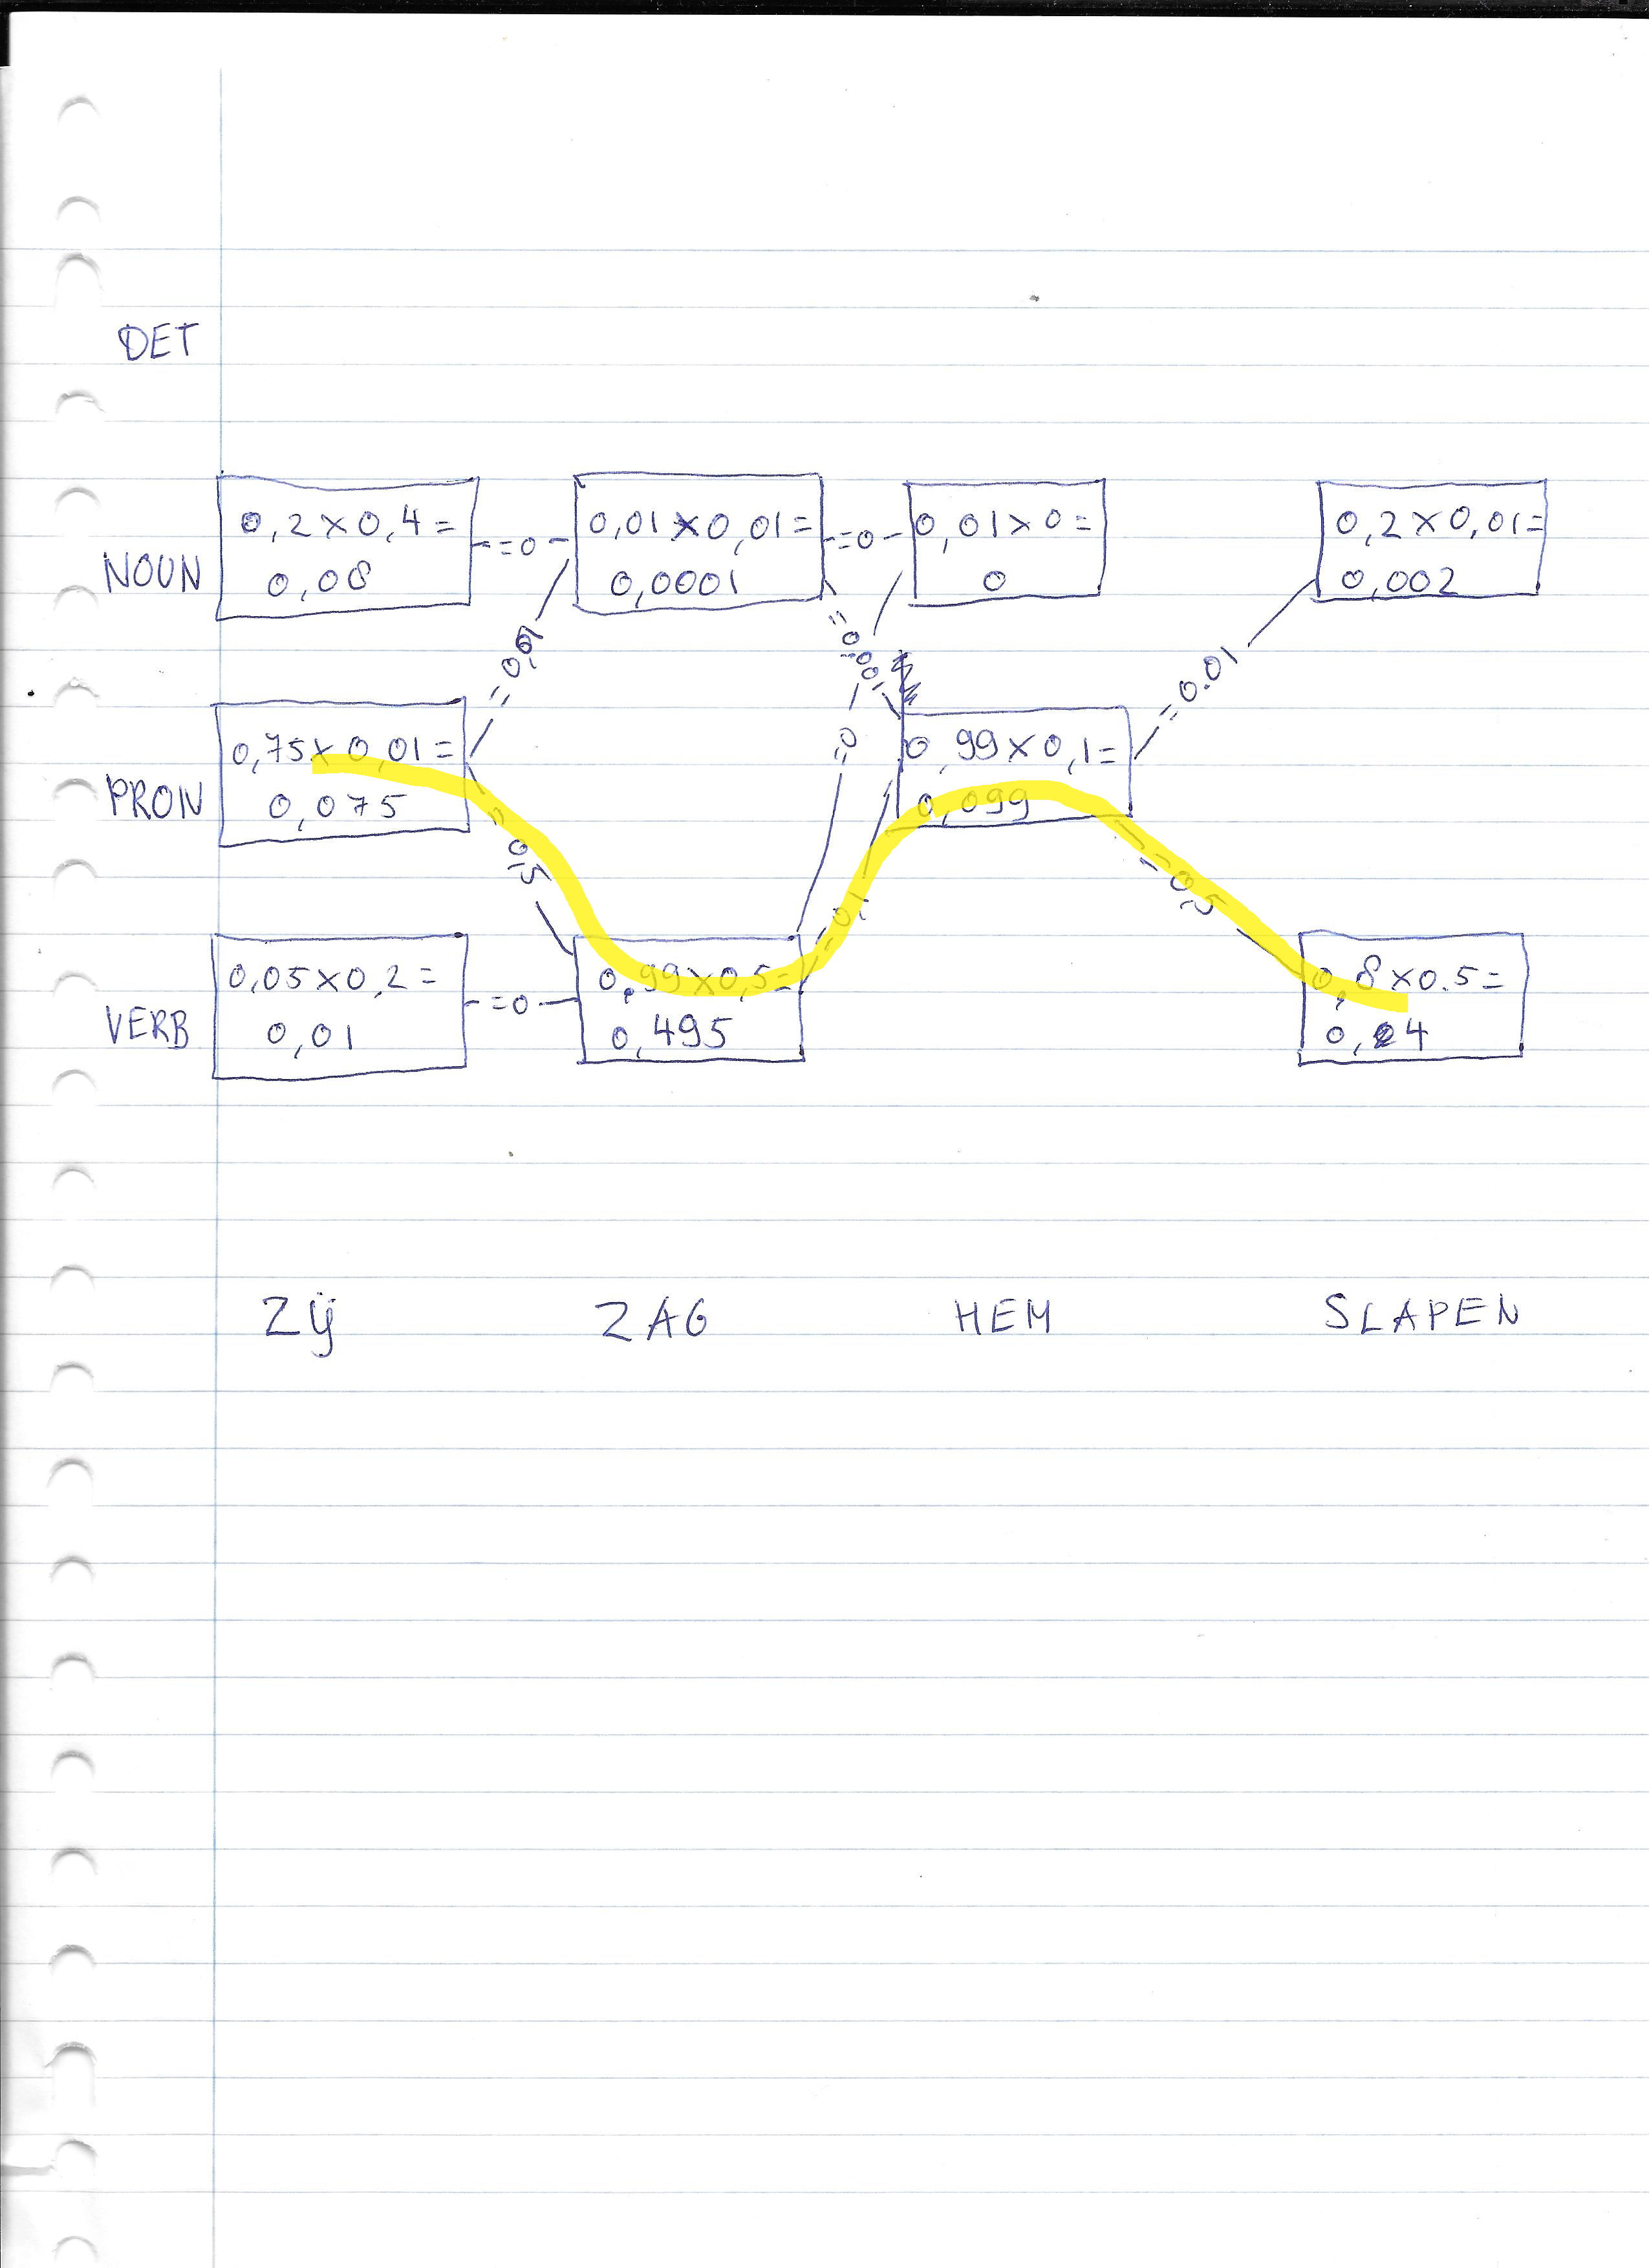
\includegraphics[width=\textwidth]{viterbi.png}
\end{figure}


\end{document}
